\documentclass[runningheads,a4paper]{llncs}
\usepackage{amssymb}
\setcounter{tocdepth}{3}
\usepackage{graphicx}
\usepackage{url}
\usepackage{epsfig}
\usepackage{algorithm}   % for pseudo-code
\usepackage{algpseudocode}     % for pseudo-code
\usepackage{amsmath}
\renewcommand{\algorithmicrequire}{\textbf{Input:}}  %for pseudo-code, Use Input in the format of Algorithm
\renewcommand{\algorithmicensure}{\textbf{Output:}} %for pseudo-code, Use Output in the format of Algorithm
\newcommand{\keywords}[1]{\par\addvspace\baselineskip
\noindent\keywordname\enspace\ignorespaces#1}

\begin{document}

%\mainmatter  % start of an individual contribution

% first the title is needed
\title{ Three Dimensional Sound Reproduction in Vehicles Based on Data Mining Techniques }
 % 基于数据挖掘技术的车内3D声场重建技术
% a short form should be given in case it is too long for the running head
% \titlerunning{Lecture Notes in Computer Science: Authors' Instructions}

% the name(s) of the author(s) follow(s) next
%
% NB: Chinese authors should write their first names(s) in front of
% their surnames. This ensures that the names appear correctly in
% the running heads and the author index.
%
\author{Maosheng Zhang, Ruimin Hu, Lin Jiang, Xiaochen Wang}
% \thanks{Project imformation}
%
% \authorrunning{Lecture Notes in Computer Science: Authors' Instructions}
% (feature abused for this document to repeat the title also on left hand pages)
% the affiliations are given next; don't give your e-mail address
% unless you accept that it will be published
\address{National Engineering Research Center for Multimedia Software\\
School of Computer Science \\
Wuhan University, Bayi road, Wuhan, China\\
}
%

\maketitle

\begin{abstract}
Three-dimension(3D) audio reproduction is a hot topic in sound reproduction system since MPEG proposed a demand . 

  This study shows a 3D sound reproduction system for vehicle. A stepwise linear regression is proposed to reproduce the sound pressure. The residuals including craw residuals, Pearson Residuals, Studentized residuals and Standardize residuals are rather small. The experiments show whatever the data volume is, the proposed reproduction system accurately simulates the theoretical reproduction system.

contain at least 70 and at most 150 words.

Three-dimension(3D) audio reproduction techniques reproduce realistic sound sources and spatial perception for listeners. The reproduction method in down-mixing system for 22.2 multichannel system aims at maintaining both sound pressure and particle velocity at listening point. In this paper, We confirm in theory that sound energy is not maintained, which leads to the loss of distance cue. To maintain the two sound physical properties, we analyse the reason of error and propose a maintenance model under some conditions. Beyond these conditions, an optimization model is used to minimize sound energy error. Subjective experiments are executed to assess the spatial reproduction performance in a real environment and objective experiments are performed in simulated scenarios. Both the subjective and objective experiments show the proposed method improves the spatial perception of sound events.

\emph{abstract} environment.
\begin{keyword}
  Vehicles, sound, data mining, reproduction
  \end{keyword}
%\keywords{Vehicles, sound, data mining, reproduction}
\end{abstract}


\section{Introduction}\label{sec:Intro}
%汽车音频研究
Sound systems for vehicle have been well researched by scientists and engineers.   Akitoshi Yamada developed a sound reproduction system for vehicle using only a pair of loudspeakers in 1982\cite{Akito82}. The system comprised a transfer function, a delay circuit, and a reverberation circuit. With the help of these components, a surrounding sound system was implemented.
Honda Motor designed a sound reproducing apparatus for vehicle in 1990\cite{terai1990sound}. The apparatus takes advantage of a acoustic duct and a loudspeaker placing in the duct.
In 2003, Takeshi reproduced a required sound image for the specified seat with a sound system consisting of two loudspeakers for Vehicles\cite{Takeshi03}.
In addition, sound systems using more than two loudspeakers are developed to generate surrounding ambiance acoustic effects\cite{clark1998vehicle}\cite{orellana2015loudspeaker}. A sound entertainment system for determined positions in a vehicle is proposed by David in 2007. This system provides ultrasonic waves and cancels the unwanted noise\cite{David07}.
FORD Motor Company invented a multichannel sound reproduction system for vehicles and applied for a patent in 2017\cite{orellana2015loudspeaker}. The embodiments mentioned in this patent composed of several loudspeakers, including a low-frequency loudspeaker or sub-woofer, placing in pillars, door frames and vehicle roof. Obviously, the sound reproduction system for entertainment in vehicle are well researched. Lots of patents about sound reproduction in vehicle are applied by vehicle companies to recreate acoustic environment\cite{David07}\cite{Simon2005}\cite{Miriam2014}\cite{Gibson15}. However, sound spatial perception is far from satisfactory and acoustic virtual reality has not been implemented in vehicle. Three-dimensional (3D) sound reproduction system provides immersive perception about sound sources and thus enhances the sensation of reality\cite{AasthaTASLP11}\cite{Danilo15TMM}\cite{zms2015}. It is necessary to reproduce 3D sound to enjoy realistic acoustic environment and sound events in vehicle.

%3D音频
The most there popular 3-D sound reproduction algorithms include Wave Field Synthesis(WFS), Ambisonics and Amplitude panning. WFS is based on Huygens principle and it is able to reproduce the whole sound field and thus the real sound immersion was recreated\cite{Gergely17}. However, WFS method is not practical since there are too many loudspeakers required in WFS system. Ambisonics system reproduces the sound pressure at listening point in the center of spherical loudspeaker array. While, it is impossible to configure a spherical loudspeaker array in vehicle. Amplitude panning is a widely used sound reproduction technique due to its computational efficiency. Vector base amplitude panning (VBAP) is a popular sound reproduction technique to render the sound direction and distance. And thus VBAP is considered as a promising technique to recreate sound events\cite{Pulkki01spatial}. Unfortunately, VBAP system requires a spherical loudspeaker array, which is not satisfied in vehicle.

Though there are several methods to reproduce sound field in physics or mathematics method, the intrinsic goal of sound field reproduction is to reproduce sound pressure at every point in the listening field. Obviously, this is a typical data mining problem. In this paper, a regression algorithm is proposed to reproduce 3D sound in a specific location, the driving seat for example. A sound pressure data set is set up at the specific listening point based on physical sound theory. The sound pressure is related to the number of loudspeakers, the location of loudspeakers, frequency of sound, the distances between listening point and loudspeakers. Since both inputs and outputs are known, a supervised learning model is built to demonstrate the relationship between received sound pressure and the all factors. The mean square error (MSE) shows the proposed regression model predicts sound pressure accurately.

The rest of this paper is organized as follows: the theory foundation, including 3D sound filed reproduction method and regression model, is introduced in the next section. The proposed method to reproduce the 3D sound in vehicle is developed in section (\ref{sec:algorithm}) experiment is conducted in section (\ref{sec:experiment}). And section (\ref{sec:conclusion}) concludes this paper.


\section{Fundamental Theory}\label{sec:Fundamental}
\subsection{3D sound reproduction}
A realistic 3D sound reproduction system needs to reproduce sound pressure at the listening point or every point in a listening area. The Fourier transform of sound pressure generated by a sound source is shown in equation (\ref{eq:SoundPressure}) \cite{zms2015}\cite{Ando11TASLP}\cite{WS13ICME}.
\begin{equation}\label{eq:SoundPressure}
p(r,\xi)=G\frac{e^{-ik|r-\xi|}}{|r-\xi|}s(\omega)
\end{equation}
where the parameters are explained as follows:\\
$\xi$: $\xi=(\xi_x\ \xi_y\ \xi_z)$ is sound source location;\\
$e$: a constant irrational number which is the base of natural logarithm;\\
$i$: imaginary unit;\\
$k$: wave number, which is equal to $\frac{2{\pi}f}{c}$;\\
$f$: sound frequency; \\
$c$: sound velocity;\\
$G$: a constant number which represents the proportionality coefficient between sound pressure at a unit distance from a loudspeaker and the input to the loudspeaker;\\
$s(t)$: sound signals in time domain; \\
$s(\omega)$: sound signals in frequency domain, i.e. Fourier transformation of sound signal $s(t)$;\\
$r=(x,\ y,\ z)$: listening point.

Alternatively, the sound pressure is also can be calculated in polar coordinates. Taking the listening point as an origin, sound pressure is shown in equation (\ref{eq:SoundPressureInPolar}).

\begin{equation}\label{eq:SoundPressureInPolar}
p(\omega)=G\frac{e^{-ik\sigma}}{\sigma}s(\omega)
\end{equation}

where $\sigma$ is the distance between sound source and listening point(the origin in polar coordinates).

It is concluded sound pressure is related to several factors after analyzing the sound pressure formula. In a multichannel reproduction system, the computational complexity grows with a exponential trend as the number of loudspeakers increases. However, whatever the 3D sound reproduction methods are, the ultimate goal of the reproduction is to recreate the sound pressure at listening point. As long as the volume of sound pressure data is large enough, data mining technology is a appropriate method to predict sound pressure.


\subsection{Regression algorithm}
Regression methods, popular techniques to predict system outputs, are well researched by scientists and engineers. Linear regression is one of the most well-known regression algorithm\cite{Hahne14Linear}\cite{Peter15The}. A linear equation is constituted by the product of a constant and  a single variable with the power of either one or zero. A typical example of linear equation is shown in equation (\ref{eq:lineareq}).
\begin{equation}\label{eq:lineareq}
    a_1x_1+a_2x_2+\dots+a_nx_n+b=0
\end{equation}

where $ a_i,i=1,2,\dot,n $ is a coefficient and $b$ is a constant.

if $a_2=a_3=\dots=a_n=0$, in other words, if there is only one variable, equation (\ref{eq:lineareq}) is the simplest linear equation, which is written as shown in equation (\ref{eq:simplestlineareq}).

\begin{equation}\label{eq:simplestlineareq}
    ax+b=0
\end{equation}

where $ a, b$ are constants.

Linear regression is a linear approach to demonstrate the relationship between inputs $X=(x_1,\ x_2, \dots, \  x_n)$ and output $Y$. In mathematics, the relationship is shown in equation (\ref{eq:LinRegression})\cite{Colin15applied}.

\begin{equation}\label{eq:LinRegression}
    y=a_1x_1+a_2x_2+\dots+a_nx_n+b
\end{equation}\label{eq:LinRegression}

In data mining, given the known dataset X and Y, the linear regression is established as shown in equation (\ref{eq:LinRegressionY}).

\begin{equation}\label{eq:LinRegressionY}
    y_i=a_1x_{i1}+a_2x_{i2}+\dots+a_nx_{in}+b_i
\end{equation}\label{eq:LinRegressionY}

In practice, matrix form is used to show the relationship, which is shown in equations (\ref{eq:LinRegressionVector1}) and (\ref{eq:LinRegressionVector2}).

\begin{equation}\label{eq:LinRegressionVector1}
    y_i=x_i^TA+b_i
\end{equation}\label{eq:LinRegressionVector1}

\begin{equation}\label{eq:LinRegressionVector2}
    Y=X^TA+B
\end{equation}\label{eq:LinRegressionVector2}

where $Y=(y_1, y_2, \dots, y_n)$, $B=(b_1, b_2, \dots, b_n), A=(a_1, a_2, \dots, a_n)$.

For given data $X$ and $Y$, the parameters, i.e. coefficients vector $A$ and constant vector $B$, are to be solved. As soon as the parameters are determined, equation (\ref{eq:LinRegressionVector2}) is able to be used as a predictor functions to predict Y according given data X.

Linear regression get widely practical uses in lots of areas such as engineering\cite{Rice04a}\cite{Vincent13determinants}, biological\cite{Vieira2016On}, epidemiology\cite{Paul13a}, finance\cite{Vincent13determinants}, economics\cite{Ehrenberg08}, environmental science\cite{piegorsch2005analyzing}, computer vision\cite{Xiujuan07locally}. Regression is also applied in acoustic science, especially in speaker recognition, emotion recognition, scenario recognition, audio event detection, audio information retrieval\cite{Alina14detecting}\cite{Zhao15invest}\cite{chen14linear}.

\section{three dimensional sound reproduction algorithm in Vehicle}\label{sec:algorithm}
First of all, a sound pressure dataset is needed. In vehicle, several loudspeakers are placed around the vehicle. The sound system is a typical multichannel sound reproduction system. The sound pressure at listening point in a multichannel sound system is the superposition of all active loudspeakers, which is shown in equation (\ref{eq:MultiSoundPressure1}).

\begin{equation}\label{eq:MultiSoundPressure1}
p(\omega)
=G\Big(\sum\limits^{L}_{j=1}\frac{e^{-ik\sigma_j}}{\sigma_j}\Big)s_j(\omega) \\
\end{equation}

where $L$ is the number of loudspeakers, $s_j(\omega)$ is sound signal in frequency domain in the $j$th loudspeaker, $sigma_j$ is the distance between the $i$th loudspeaker and the origin.

The purpose of a 3D sound reproduction system in vehicle is to reproduce the same sound pressure at listening point in vehicle using several loudspeakers as the sound pressure the sound source generated. Given the received signal s(t) in time domain, we need to reproduce s(t) in loudspeaker array. In an amplitude panning system, the sound signal in the $j$th loudspeaker is assigned as $ s_j(\omega)=w_is(\omega)$, where $w_j$ is the $j$th weight. And then, equation (\ref{eq:MultiSoundPressure1}) is equivalently transformed to equation (\ref{eq:MultiSoundPressure2}).

\begin{equation}\label{eq:MultiSoundPressure2}
p(\omega)
=G\Big(\sum\limits^{L}_{j=1}\frac{e^{-ik\sigma_j}}{\sigma_j}\Big)w_js(\omega) \\
\end{equation}

Apparently, it is necessary to solve all the weights $w=(w_1,w_2,\dots,w_L)$ in equation (\ref{eq:MultiSoundPressure2}).  Unfortunately, it is hard to get a accurate solution to maintain sound pressure. Since sound pressure is depend on several factors and $w_i$ is ranged from $0$ to $1$, regression model is an efficient method to estimate sound pressure as soon as a large amount of sound pressure data is available.

Sound pressure dataset is created with parameters sound signal frequency $f$, the $i$th loudspeaker location $L_i=(\theta_i,\delta_i,\sigma_i)$, listening point location $O$ and $ W=(w_1,w_2,\dots,w_L) $ based on equation (\ref{eq::MultiSoundPressure2}), where  $\theta_i,\delta_i$ is azimuth and elevator of the $i$th loudspeaker respectivly, $w_i$ ranges from $0$ to $1$ with step-size $ h $. Let every $w_i$ traverses all the possible values and we calculate the corresponding sound pressure, a big sound pressure dataset is created. The data size of this dataset is shown in equation (\ref{eq:datasize}).

\begin{equation}\label{eq:datasize}
    V=f_b \times L^(1/h)
\end{equation}\label{eq:datasize}

where $f_b$ is the number of frequencies.

It is obvious that the smaller the step-size $ h $ is, the larger the dataset is, and the  more accurate the regression model is. Assuming there are five loudspeakers in a vehicle and step-size $h=0.01$, there are $7.8886*10^69$ sound pressure values for each frequency. When we design program algorithm, the generating of each $w_i$ is randly chosen by a rand function rather than a fixed step-size since the weights in reality is barely uniform. There is another constraint for weight vector where every $w_i$ is non-negative and the sum of all elements in $W$ is 1. The sound pressure dataset generating algorithm is shown in algorithm (\ref{alg:SPdatasetGen}).

\begin{algorithm}[htb]
    \caption{ Framework of generating sound pressure dataset.}
    \label{alg:SPdatasetGen}
    \begin{algorithmic}[1]
      \Require   \\ % Input
        sound signal frequency $f$;  \\
        the loudspeaker location $L_i=(\theta_i,\delta_i,\sigma_i),i=1,2,\dots,L$;  \\
        listening point location $O$;

      \Ensure    \\ %output
        a dataset SPdata composed of sound pressure $p$, weight vector $W$ and the above mentioned inputs;
      \State loop variable i=0;
      \label{code:generateW}
      \State generating weight vector;
      \State i=i+1;
      \State estimating sound pressure p;
      \label{code:estimateP}
      \State pushing sound pressure and parameters into dataset SPdata ;
      \label{code:pushdataset}
      \State if $i \leq v$ then goto state (\ref{code:generateW});  else goto state (\ref{code:return}); \\
      \Return SPdata;
      \label{code:return}
    \end{algorithmic}
  \end{algorithm}

  Since a sound pressure dataset is created, a stepwise linear regression model is going to be established. Taking parameters $f$, $L_i=(\theta_i,\delta_i,\sigma_i)$, $O$ and $ W=(w_1,w_2,\dots,w_L) $ as predictors and sound pressure $p$ as response, a linear regression model is proposed. In order to protect against over-fitting, we also design cross-validation technique by partitioning the dataset into 5 folds and estimating accuracy on each fold. When the training and cross validation are finished, the prediction function is determined and can be used to predict new data. Figure (\ref{fig:ModelFlowchart}) shows the flowchart of the developed sound reproduction regression model.
% --------------------------------to be finised: 流程图
  \begin{figure}[htb]
    \centering
    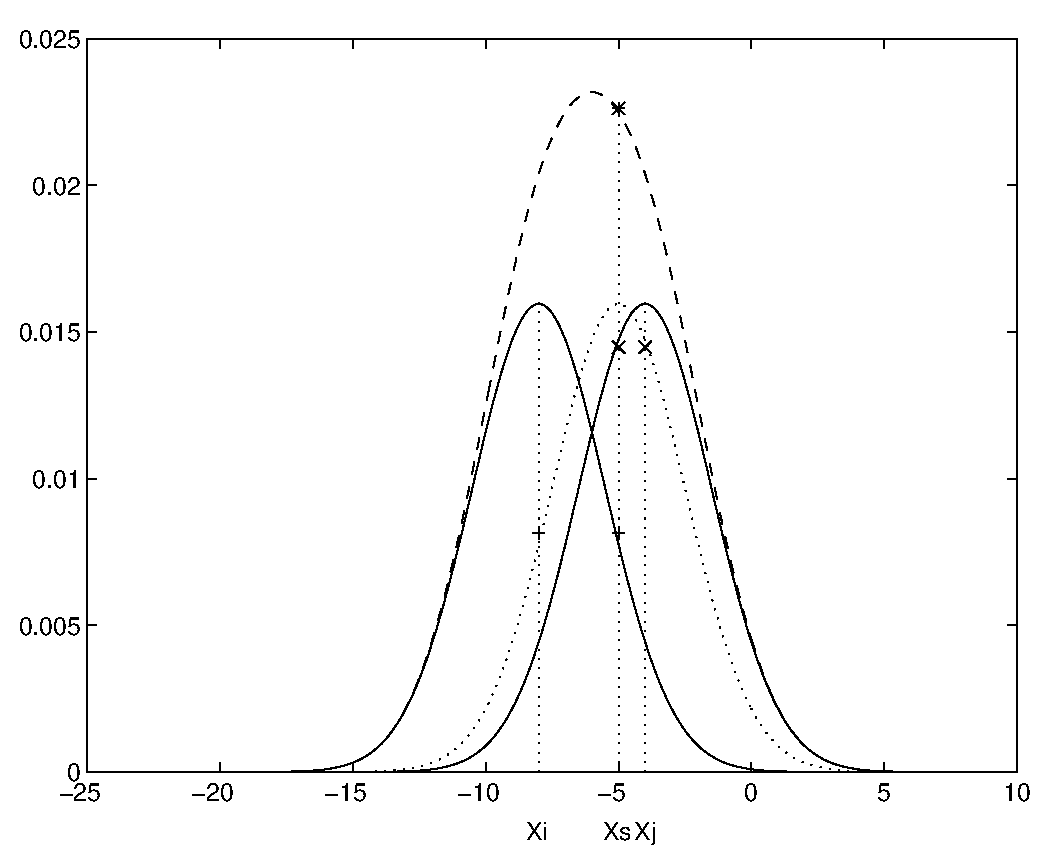
\includegraphics[width=11.5cm]{888.eps}
    \caption{The flowchart of the sound reproduction regression model in vehicle}
    \label{fig:ModelFlowchart}
  \end{figure}

% 生成理论的声压数据库
% 对数据库进行训练
% 得到模型并用于预测
% 分析误差表现
Getting loudspeaker array parameters
Generating sound pressure dataset
% data mining
partitioning dataset
Training
cross validation
prediction

%

\section{program and experiment}\label{sec:experiment}
\subsection{implementation}
We utilize Matlab 2017 to train the proposed model and analyze the model performance. The number of the loudspeaker array is $4$. We assume the four loudspeakers are placed at left front($L_1$), right front($L_2$), right behind($L_3$) and left behind($L_4$). The location coordinates of all loudspeakers are shown in table (\ref{tab:LPLocation}).

\begin{table}[htbp]
  \caption{\label{tab:LPLocation}Loudspeakers location}
  \centering
  \begin{tabular}{|c | c| c|}
    \hline
    loudspeaker           & azimuth     & elevator        \\
    \hline
    L1                 & $320^{\circ}$     & $0^{\circ}$    \\
    L2                 & $80^{\circ}$       & $0^{\circ}$    \\
    L3                 & $135^{\circ}$     & $0^{\circ}$      \\
    L4                 & $225^{\circ}$     & $0^{\circ}$       \\
    \hline
  \end{tabular}
\end{table}


The proposed model is programmed on a notebook manufactured in 2011. The hardware parameters are shown in table (\ref{tab:Hardware}).

\begin{table}[htbp]
    \caption{\label{tab:Hardware} Notebook hardware parameters}
    \centering
    \begin{tabular}{|c | c|}
      \hline
      Item           & Parameter value             \\
      \hline
      CPU                 & i7 3610QM, 2.30GH       \\
      RAM                 & 4G       \\
      system                 & windows 10     \\
      \hline
    \end{tabular}
\end{table}



It takes 33.3 seconds to finish the regression model and vital parameters of the stepwise linear regression model is shown in table (\ref{tab:parametersinRegression}).

Regression model parameters in table (\ref{tab:parametersinRegression}) indicate the proposed model for 3D sound reproduction in vehicle is accurate since both the MSE, RMSE are rather small. Due to the poor performance of the notebook, the prediction speed is slow and the training time is long.

\begin{table}[htbp]
    \caption{\label{tab:parametersinRegression}Parameters in subjective experiments}
    \centering
    \begin{tabular}{|c | c|}
    \hline
    Parameter           & value                 \\
    \hline
    MSE                 & 7.9968e-19            \\
    RMSE                & 8.9425e-10            \\
    R-squared           & 1                     \\
    DFE                 & 9996                  \\
    SSE                 & 7.9936e-15            \\
    SST                 & 3.9626                \\
    SSR                 & 3.9626                \\
    MAE                 & 0                     \\
    Prediction speed    &   130000 obs/sec      \\
    Training time       &   33.306 sec          \\
    \hline
    \end{tabular}
    \end{table}


  We also demonstrate the residuals in our model. The raw residuals, Pearson residuals, studentized residuals, standardized residuals is illustrated in figures (\ref{fig:RawResiduals})-(\ref{fig:standardized}) respectively. The tiny residuals shown int figures (\ref{fig:RawPearsonResiduals})-(\ref{fig:ssResiduals}) concisely presents the accuracy on 3D sound reproduction.


  \begin{figure}[bth]
    \begin{minipage}{0.28\linewidth}
      \centerline{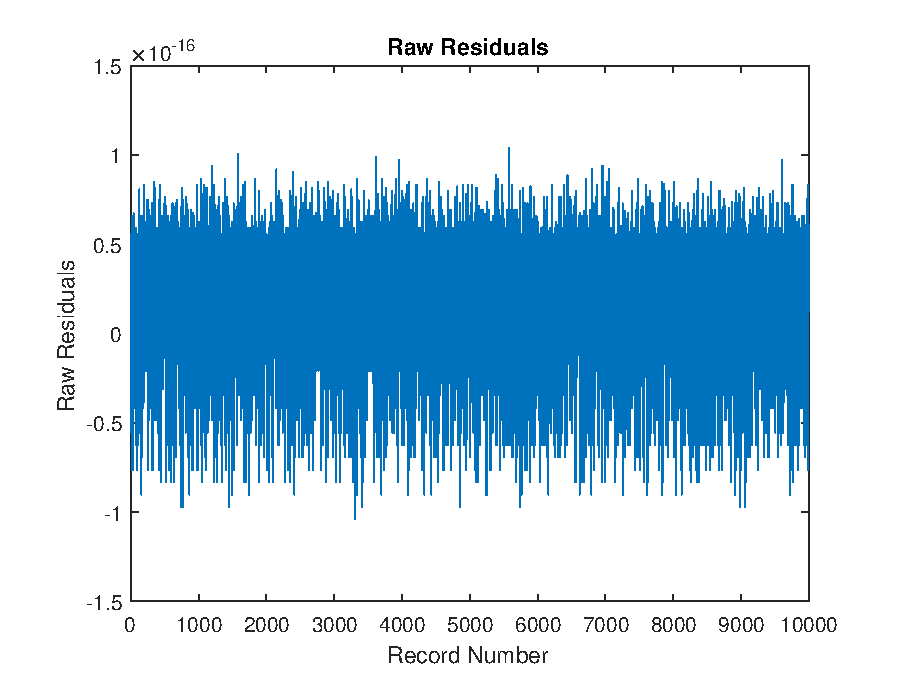
\includegraphics[width=8.5cm]{Residuals_Raw.eps}}
      \centerline{(a) Raw residuals}
    \end{minipage}
    \hfill
    \begin{minipage}{.28\linewidth}
      \centerline{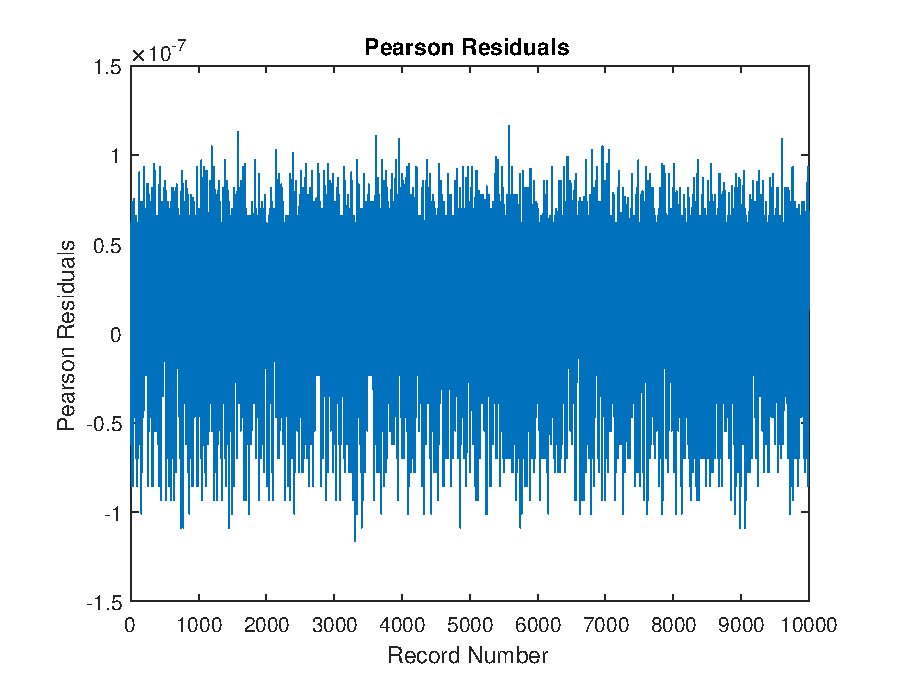
\includegraphics[width=8.5cm]{Residuals_Pearson.eps}}
      \centerline{(b) Pearson residuals}
    \end{minipage}
    \caption{Raw residuals and c}
    \label{fig:RawPearsonResiduals}
  \end{figure}

  \begin{figure}[bth]
    \begin{minipage}{0.28\linewidth}
      \centerline{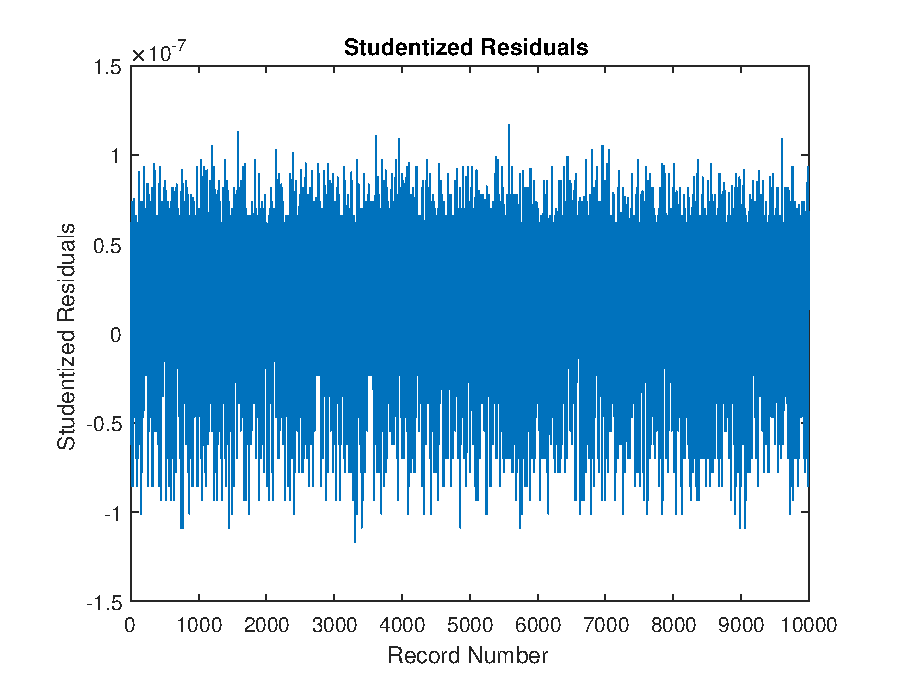
\includegraphics[width=8.5cm]{Residuals_Studentized.eps}}
      \centerline{(a) Studentized residuals}
    \end{minipage}
    \hfill
    \begin{minipage}{.28\linewidth}
      \centerline{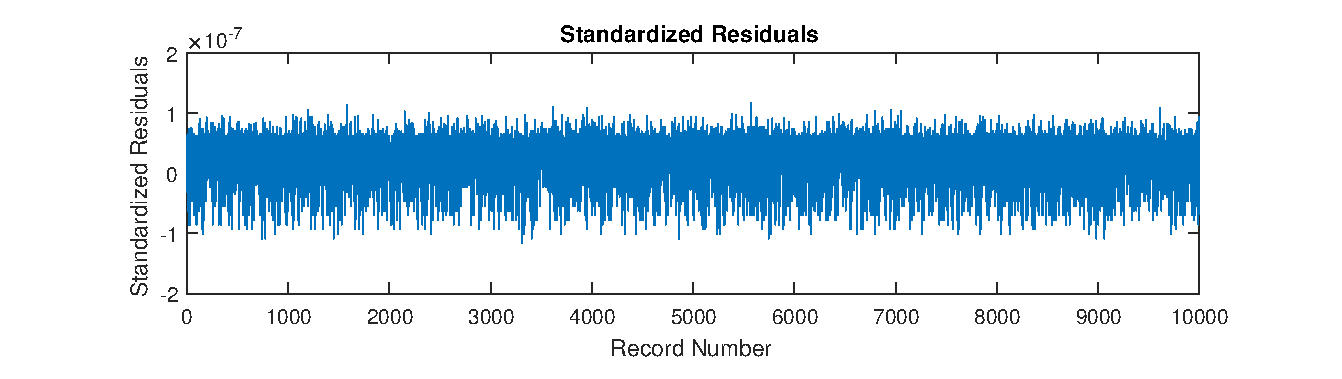
\includegraphics[width=8.5cm]{Residuals_Standardize.eps}}
      \centerline{(b) Standardize residuals}
    \end{minipage}
    \caption{Studentized residuals and Standardize residuals}
    \label{fig:ssResiduals}
  \end{figure}

%----------------to be finished: experiment
\subsection{experiment}
We conducted three experiments to evaluate the reproduction performance of the proposed technique. The result are compared with sound pressure in theory. The less residuals the proposed method are, the more accurate the reproduction method is. The loudspeaker configuration in the experiments is in shown in  table (\ref{tab:LPLocation}). In order to verify the over fitting and under fitting performance, different data volume was under test. In experiment $1$, we tested $100$ sound pressure while in the other two experiments $1000$ and $10000$ computations are conducted. We randomly generated different weights in each computation. To show detailed comparison, raw residuals are represented graphically. Figures (\ref{fig:Experimentwith100data_Residuals})-(\ref{fig:Experimentwith10000data_Residuals}) show the residuals in experiments. The negligible residuals exhibite the proposed regression model accurately reproduce the sound pressure.


\begin{figure}[bthp]
  \begin{minipage}{0.28\linewidth}
    \centerline{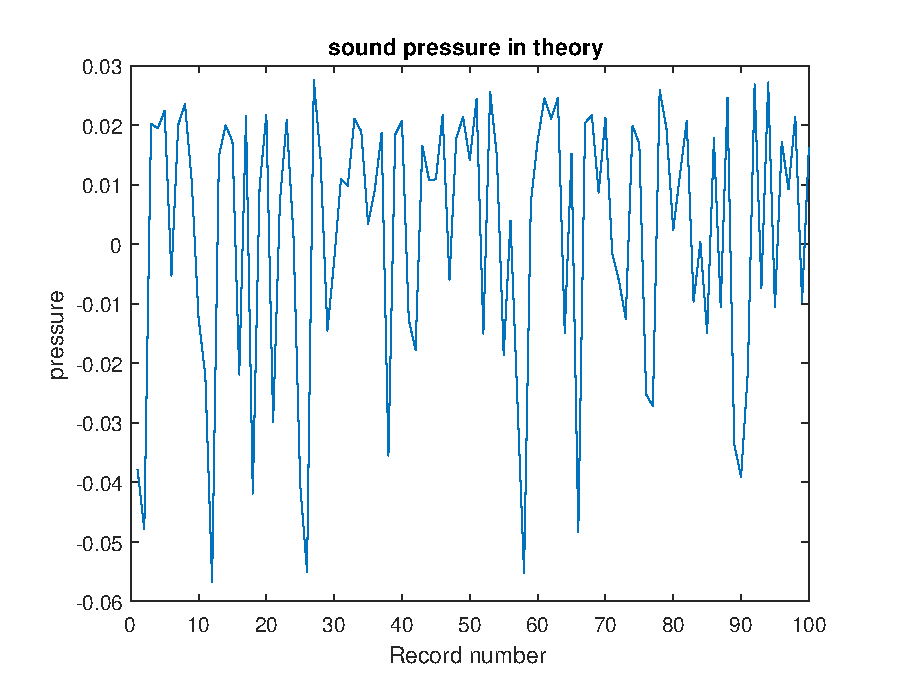
\includegraphics[width=4.5cm]{Experimentwith100data_pressure.eps}}
  %  \centerline{(a) sound pressure in theory}
  \end{minipage}
  \hfill
  \begin{minipage}{.28\linewidth}
    \centerline{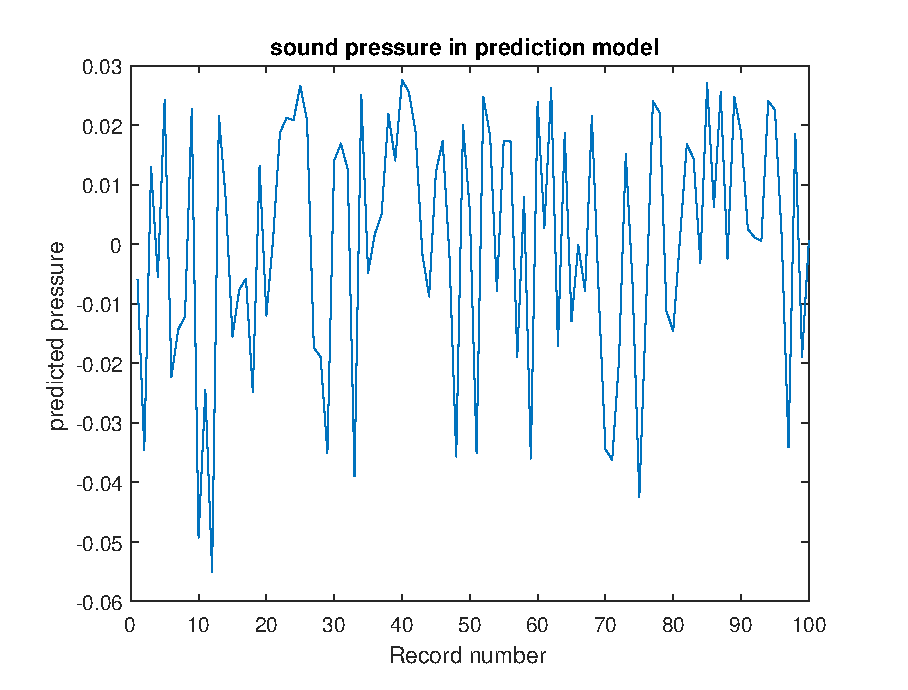
\includegraphics[width=4.5cm]{Experimentwith100data_PressurePredicted.eps}}
  %  \centerline{(b) predicted sound pressure}
  \end{minipage}
  \hfill
  \begin{minipage}{0.28\linewidth}
    \centerline{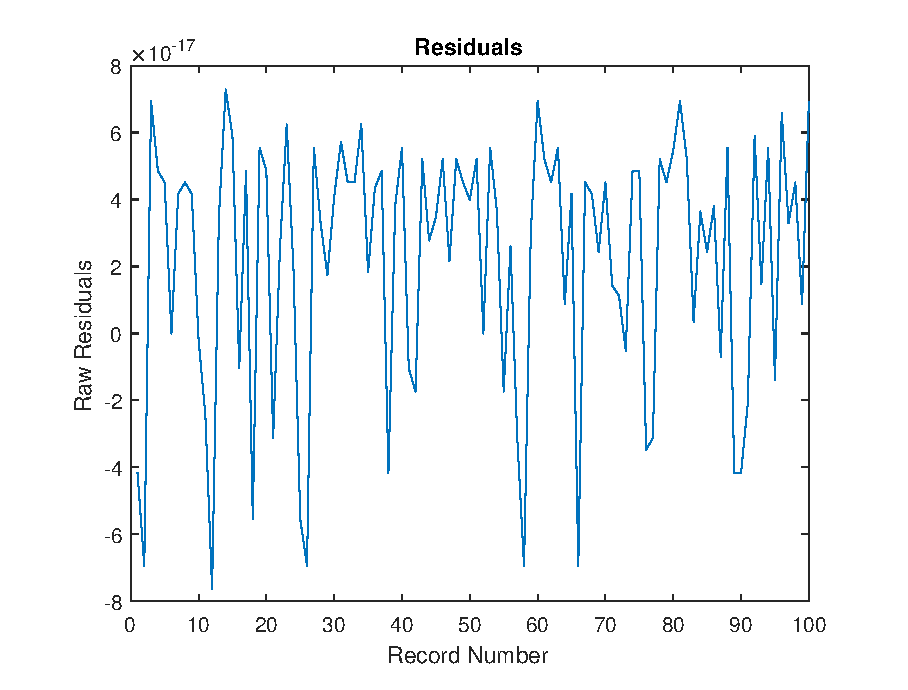
\includegraphics[width=4.5cm]{Experimentwith100data_Residuals.eps}}
  \end{minipage}
  \vfill
  \caption{prediction residuals in experiment (100 different weights)}\label{fig:250Hz}
  \label{fig:Experimentwith100data_Residuals}
\end{figure}

\begin{figure}[bthp]
  \begin{minipage}{0.28\linewidth}
    \centerline{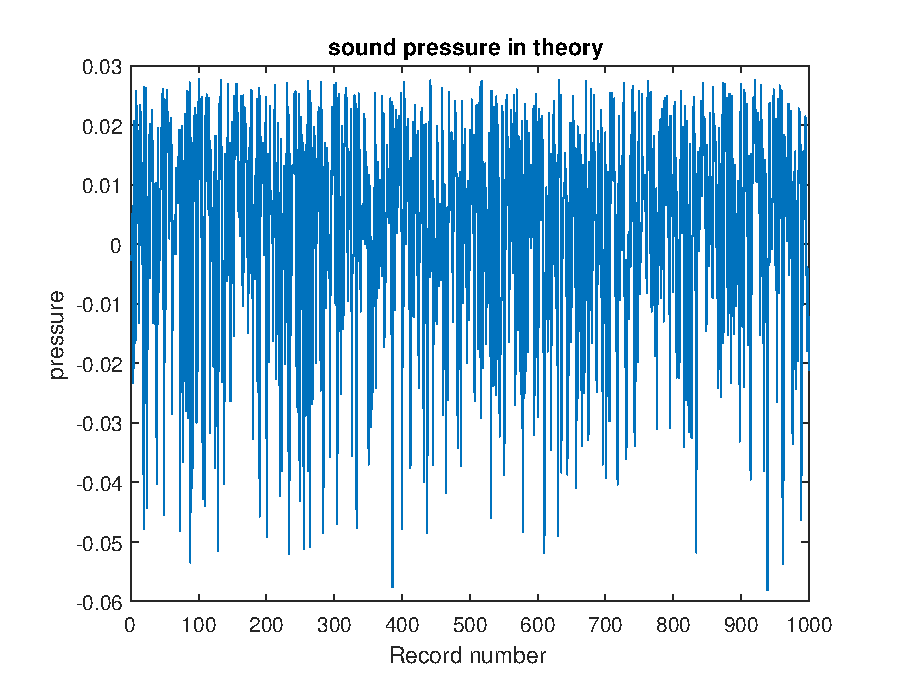
\includegraphics[width=4.5cm]{Experimentwith1000data_pressure.eps}}
  %  \centerline{(a) sound pressure in theory}
  \end{minipage}
  \hfill
  \begin{minipage}{.28\linewidth}
    \centerline{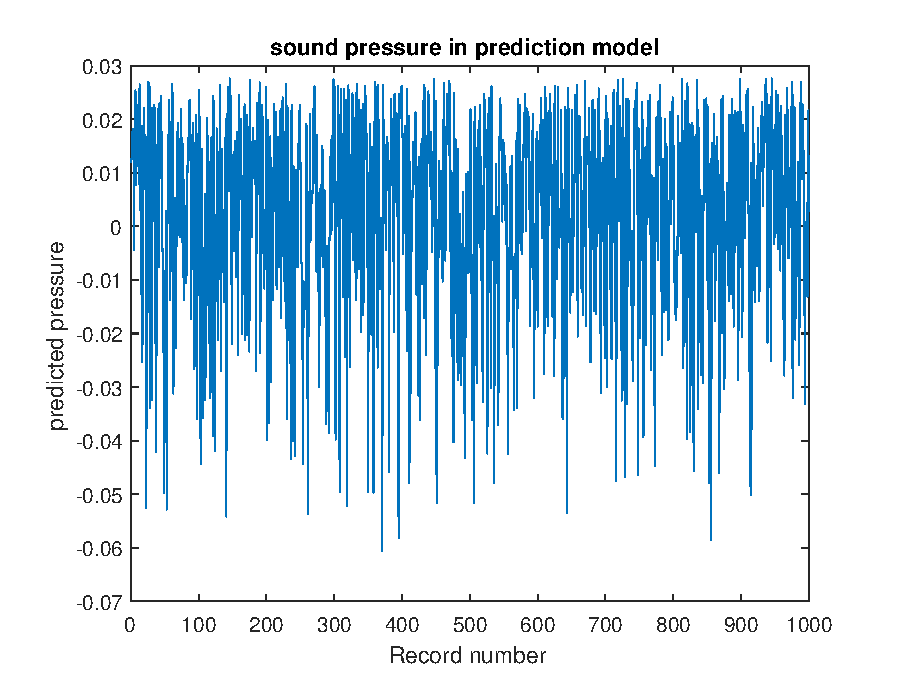
\includegraphics[width=4.5cm]{Experimentwith1000data_PressurePredicted.eps}}
  %  \centerline{(b) predicted sound pressure}
  \end{minipage}
  \hfill
  \begin{minipage}{0.28\linewidth}
    \centerline{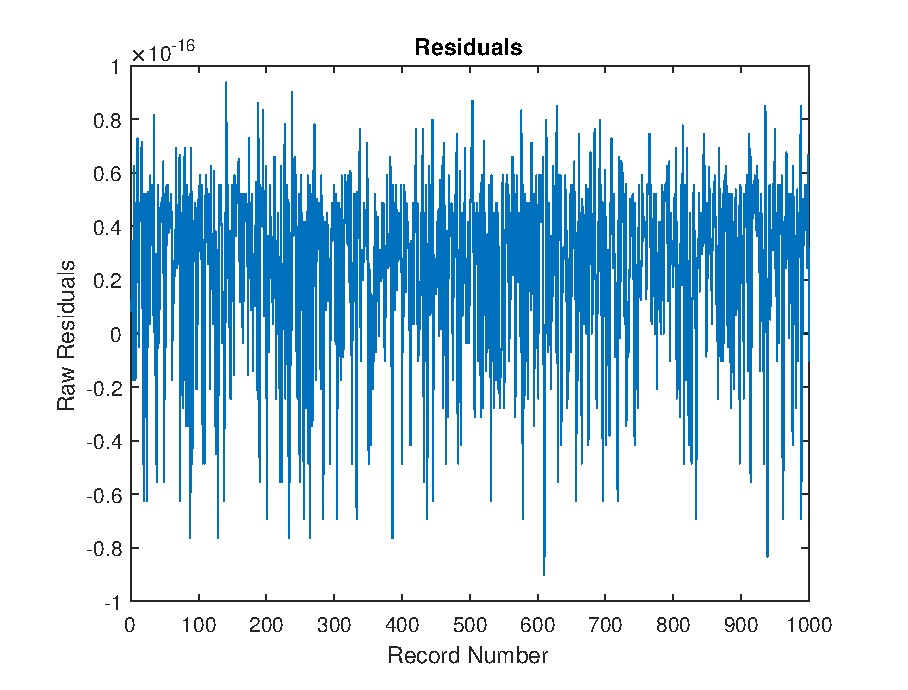
\includegraphics[width=4.5cm]{Experimentwith1000data_Residuals.eps}}
  \end{minipage}
  \vfill
  \caption{prediction residuals in experiment(1000 different weights)}\label{fig:250Hz}
  \label{fig:Experimentwith1000data_Residuals}
\end{figure}


\begin{figure}[bthp]
  \begin{minipage}{0.28\linewidth}
    \centerline{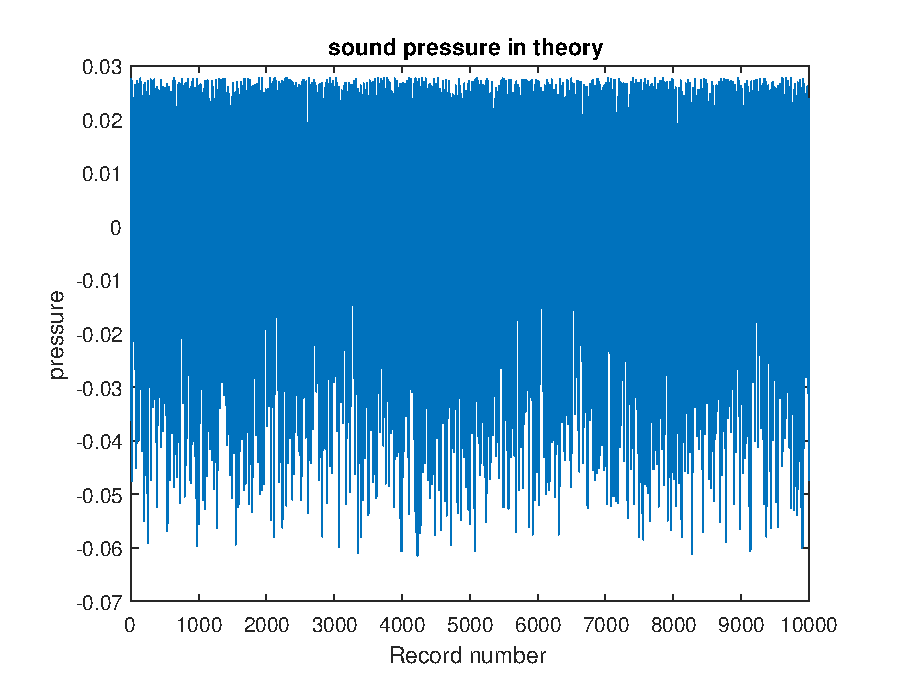
\includegraphics[width=4.5cm]{Experimentwith10000data_pressure.eps}}
  %  \centerline{(a) sound pressure in theory}
  \end{minipage}
  \hfill
  \begin{minipage}{.28\linewidth}
    \centerline{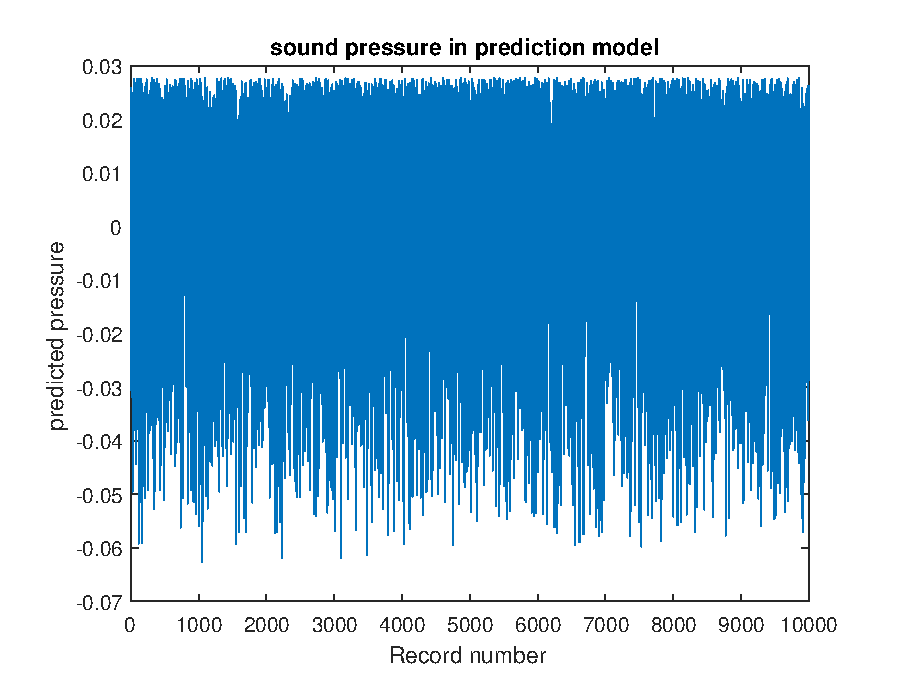
\includegraphics[width=4.5cm]{Experimentwith10000data_PressurePredicted.eps}}
  %  \centerline{(b) predicted sound pressure}
  \end{minipage}
  \hfill
  \begin{minipage}{0.28\linewidth}
    \centerline{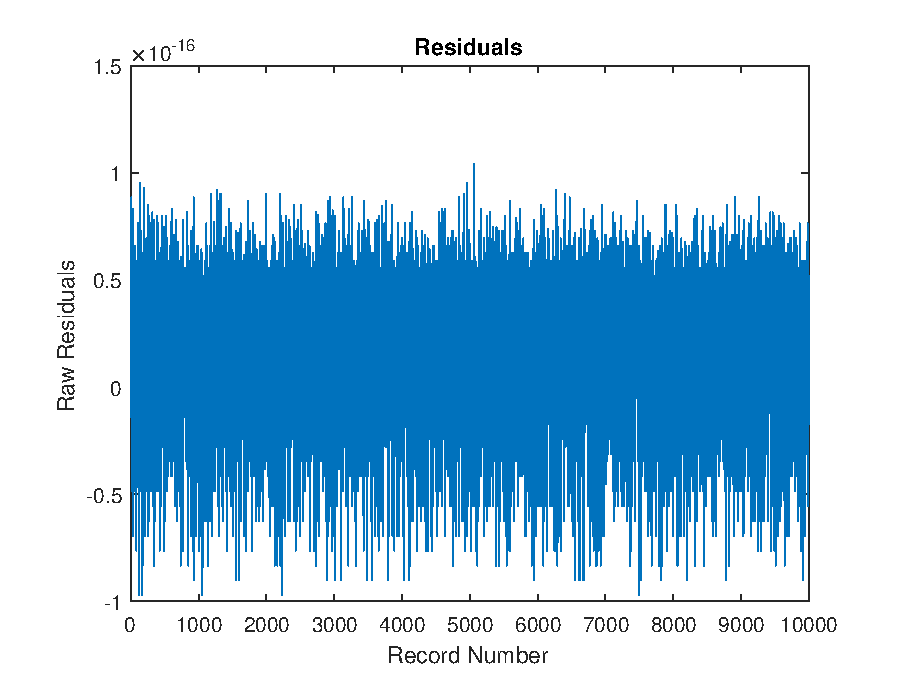
\includegraphics[width=4.5cm]{Experimentwith10000data_Residuals.eps}}
  \end{minipage}
  \vfill
  \caption{prediction residuals in experiment(10000 different weights)}\label{fig:250Hz}
  \label{fig:Experimentwith10000data_Residuals}
\end{figure}



\section{conclusion}\label{sec:conclusion}
This study shows a 3D sound reproduction system for vehicle. A stepwise linear regression is proposed to reproduce the sound pressure. The residuals including craw residuals, Pearson Residuals, Studentized residuals and Standardize residuals are rather small. The experiments show whatever the data volume is, the proposed reproduction system accurately simulates the theoretical reproduction system.

\section{ACKNOWLEDGMENT}
This research was supported by National Nature Science Foundation of China (No.61761044, 61762005, 61701194, 61471271, 61671335), National Nature Science Foundation of China (No. U1736206), Guangxi Colleges and Universityies Key Laboratory of Complex System Optimization and Big Data Processing(No.2016CSOBDP0005).

\label{bib:bibliography}
\bibliographystyle{ISIT}
\bibliography{ISIT}


\end{document}
